\begin{itemize}

\item Các mẫu chiến lược phân tích nghiệp vụ kinh doanh sau đó đưa ra việc phân chia các thành phần và hiểu mối quan hệ của các thành phần đó.

\item Các mẫu chiến lược là giai đoạn xây dựng sự hiểu biết chung về miền giữa chuyên gia ngành và nhóm phân tích hệ thống.

\begin{itemize}

\item Các mẫu chiến lược giúp xác định các thành phần quan trọng của hệ thống.

\item Các mẫu chiến lược đảm bảo kiến trúc phần mềm phản ánh đúng các yêu cầu kinh doanh.

\end{itemize}

$\Rightarrow$ Các mẫu chiến lược xác định mục tiêu tạo ra hệ thống có thể mở rộng, phát triển linh hoạt theo nhu cầu kinh doanh.

\item Các mẫu chiến lược đề cập đến thiết kế tổng thể của hệ thống bao gồm:

\begin{itemize}

\item Muc1

\item Muc2

\item các mục bên dưới \dots

\end{itemize}

\end{itemize}

\begin{figure}[H]

\centering

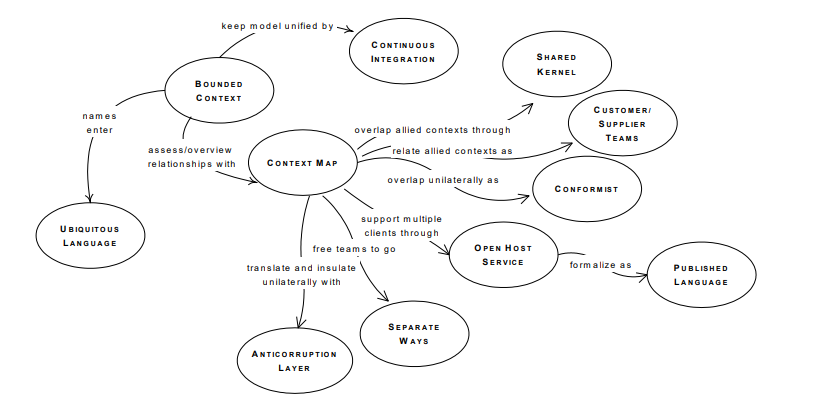
\includegraphics[width = 1\textwidth]{pictures/CacMoHinhChienLuoc/temp.png}

\caption{Sơ đồ về các thành phần trong mô hình chiến lược}

\end{figure}

%!<! - - $ Vẽ lại sau: - - >

%!<! - - $ Vẽ lại sau: - - >

%!<! - - $ Vẽ lại sau: - - >

%!<! - - $ Vẽ lại sau: - - >

%!<! - - $ Vẽ lại sau: - - >

%!<! - - $ Vẽ lại sau: - - >

%!<! - - $ Vẽ lại sau: - - >

%!<! - - $ Vẽ lại sau: - - >

%!<! - - $ Vẽ lại sau: - - >

%!<! - - $ Vẽ lại sau: - - >

%!<! - - $ Vẽ lại sau: - - >

%!<! - - Bối cảnh giới hạn (Bounded Context) - - >

%!<! - - [Giữ cho mô hình thống nhất] Tích hợp Liên tục (Continuous Integration) - - >

%!<! - - [Tính nhất quán trong trao đổi] Ngôn ngữ chung (Ubiquitous Language) - - >

%!<! - - [Tổng quan mối quan hệ] Bản đồ bối cảnh (Context Maps) - - >

%!<! - - Symmetric Relationship: Separate ways, Shared Kernel - - >

%!<! - - Asymmetric Relationship: Customer - Supplier, Conformist, Anti Corruption Layer - - >

%!<! - - - - >

%!<! - - One - to - Many Relationship: Open Host Service, Published Language - - >

%!<! - - dịch và cách ly đơn phương với - - >

%!<! - - [lớp] lớp (Context Maps) - - >

%

%!<! - - "Bản đồ bối cảnh dịch chuyển và cách ly một cách đơn phương để tạo thành cấu trúc lớp." - - >

%!<! - - Tách biệt - - >

